\chapter{Assemblaggio della scheda}

Come già accennato in precedenza, una volta finita la fase di progetto della scheda, abbiamo 
inviato al professore tutti i file relativi alla produzione (Gerber, Drill e BOM), 
il quale ha poi provveduto ad inviare le PCB in produzione, ordinando anche uno 
stencil, e ad effettuare gli ordini per i componenti necessari.\\
Dopo circa due settimane dall’invio eravamo finalmente in possesso delle schede 
e della maggior parte dei componenti necessari, quindi abbiamo potuto cominciare 
l’assemblaggio, che è stato svolto sotto la supervisione del Professore presso 
il laboratorio di elettronica del FabLab.\\
Prima di qualsiasi cosa abbiamo effettuato un’ispezione visiva delle PCB sotto 
una lente per verificarne la correttezza; grazie a questa abbiamo identificato 
un solo problema: il marker sul layer silkscreen per il pin 1 del microcontrollore 
non è stato stampato, probabilmente perché era troppo piccolo.\\
Abbiamo poi ispezionato anche lo stencil per la pasta saldante ed abbiamo notato 
che il produttore non ha usato come riferimento il layer apposito, ma ha usato 
quello per la soldermask. Per questo motivo sullo stencil erano presenti aperture 
anche in corrispondenza dei pad through-hole del gps (che abbiamo provveduto a 
coprire con del nastro kapton) e le aperture dei fiducials sono risultate più 
grandi del previsto, anche se questo non ha alcuna importanza per la realizzazione, 
quindi siamo passati allo step successivo.\\
Per iniziare l’assemblaggio abbiamo fissato una PCB con altre 4 utilizzando del 
nastro ed abbiamo allineato lo stencil fissandolo da un lato con altro nastro per 
poterlo alzare una volta finito, come in figura.

\begin{center}
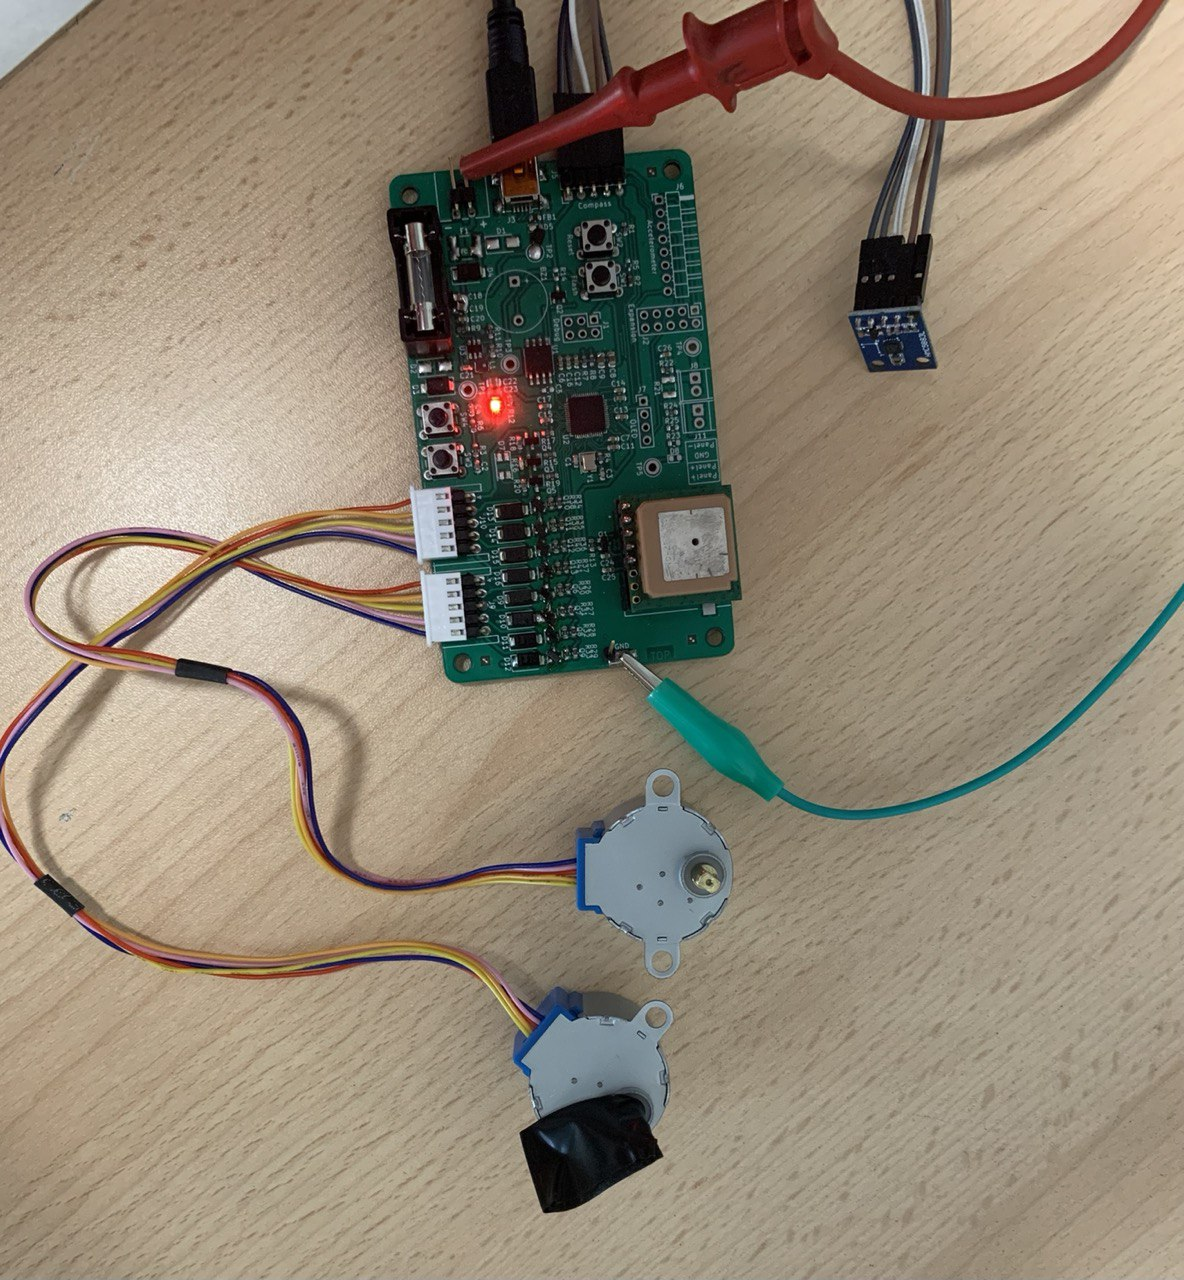
\includegraphics[scale=0.4]{figures/image101.png}
\captionsetup{type=figure}
\captionof{figure}{Scheda SALMO completa di componenti essenziali}
\end{center}

\noindent Abbiamo quindi depositato, con l’aiuto di una spatola, la pasta saldante, 
controllando di riempire ogni apertura con una quantità adeguata. Verificata la 
corretta applicazione abbiamo tolto la scheda dal supporto da noi creato ed abbiamo 
cominciato ad applicare i componenti SMD con l’aiuto di pinzette di precisione e controllando 
continuamente il layout.

\begin{center}
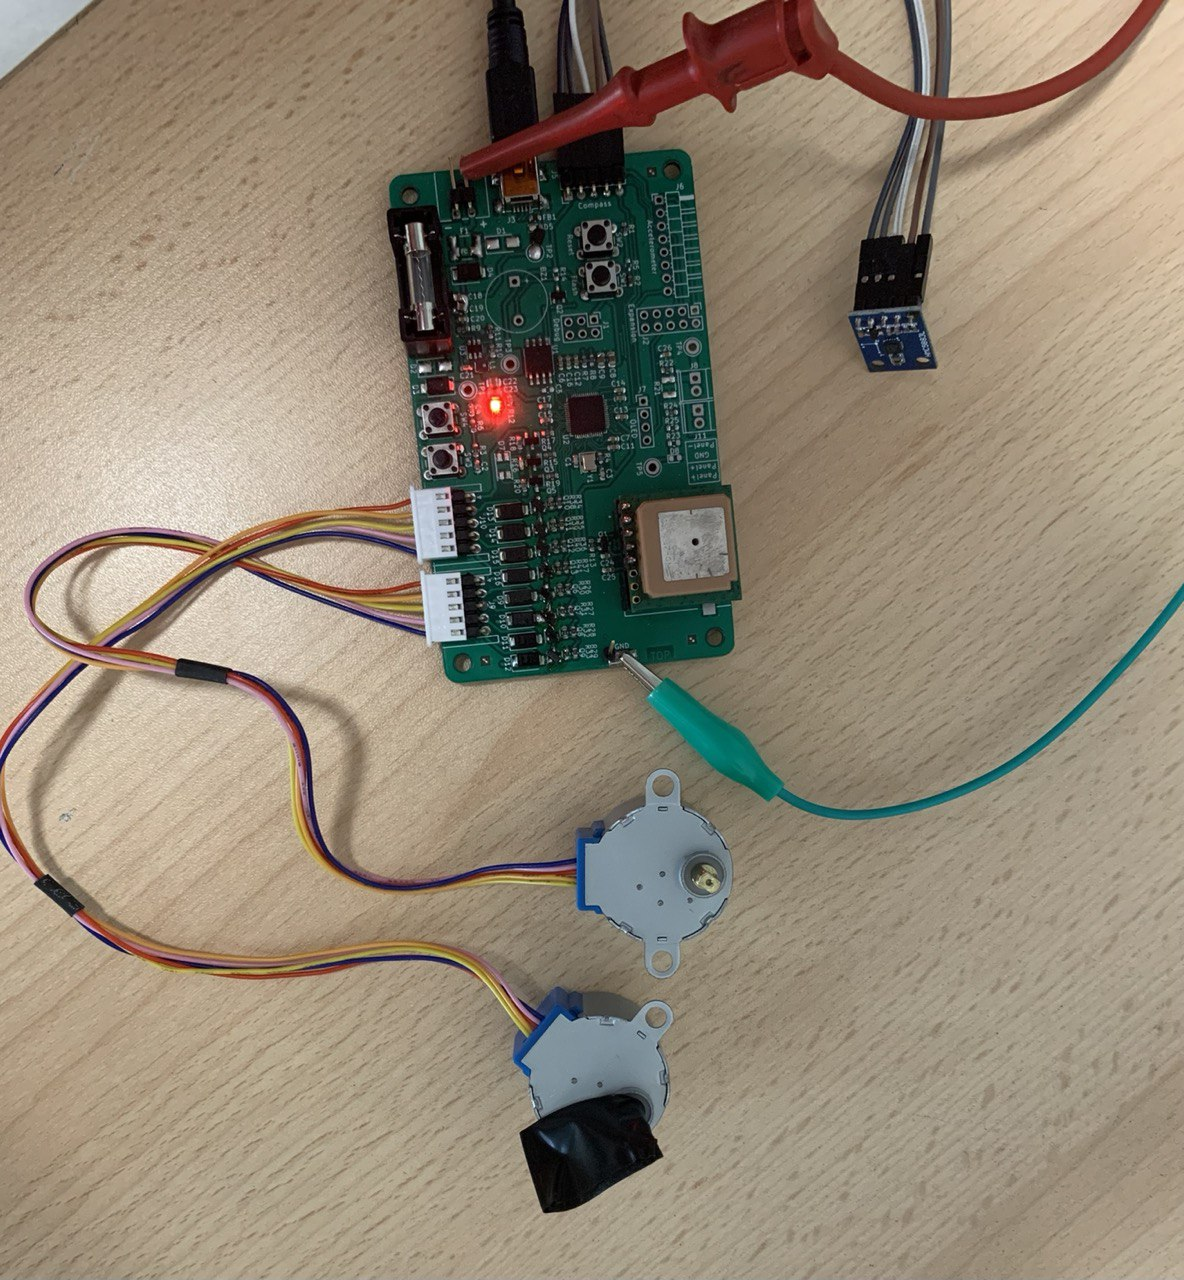
\includegraphics[scale=0.4]{figures/image101.png}
\captionsetup{type=figure}
\captionof{figure}{Scheda SALMO completa di componenti essenziali}
\end{center}

\noindent Per tenere traccia del progresso abbiamo usato estensivamente un 
utilissimo plugin per KiCad chiamato iBOM, che permette di visualizzare il 
layout del PCB, associando ad ogni componente la sua posizione in una grafica molto 
intuitiva, e di contrassegnare ogni componente come piazzato.

\begin{center}
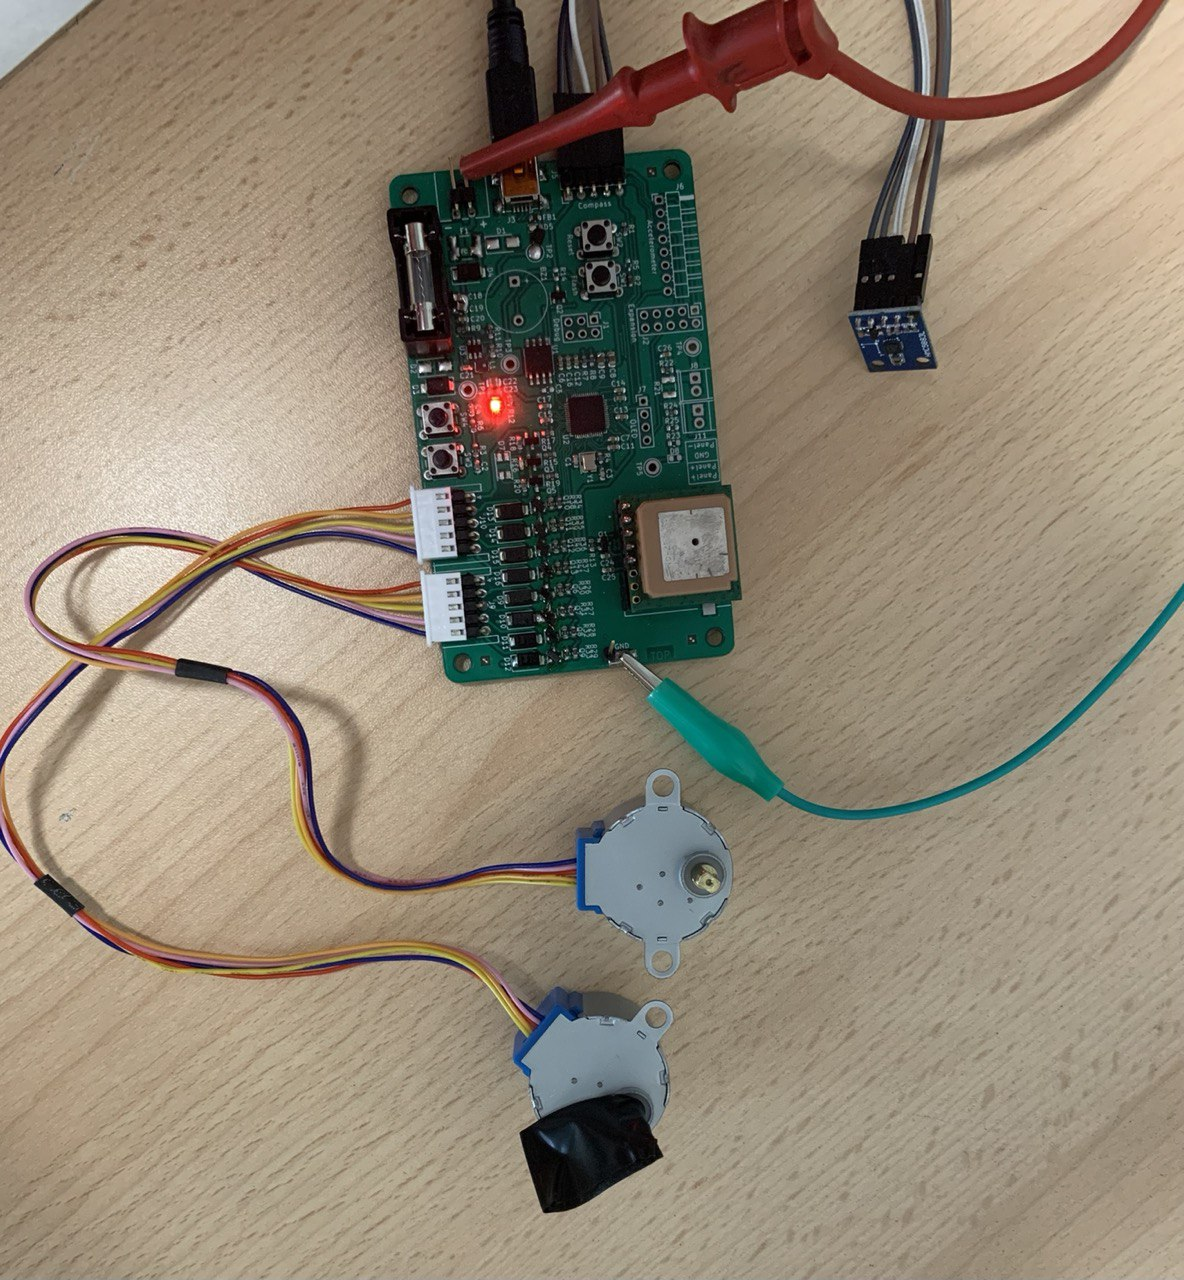
\includegraphics[scale=0.4]{figures/image101.png}
\captionsetup{type=figure}
\captionof{figure}{Scheda SALMO completa di componenti essenziali}
\end{center}

\noindent Alcuni dei componenti utilizzati presentavano un modello diverso da quello previsto
in fase di progettazione a seconda delle disponibilità in-house del professore ma, 
essendo una scheda di prototipazione e non una scheda di produzione, sono risultati 
ugualmente adatti, senza alterare il funzionamento della scheda. Infine, abbiamo posto
la scheda su di una piastra elettrica riscaldante controllata per fare il reflow della 
pasta e saldare definitivamente i componenti SMD. A questo punto abbiamo saldato manualmente, 
con un classico saldatore a stilo, i restanti componenti THT, ovvero buzzer, pulsanti, portafusibile e connettori.

\begin{center}
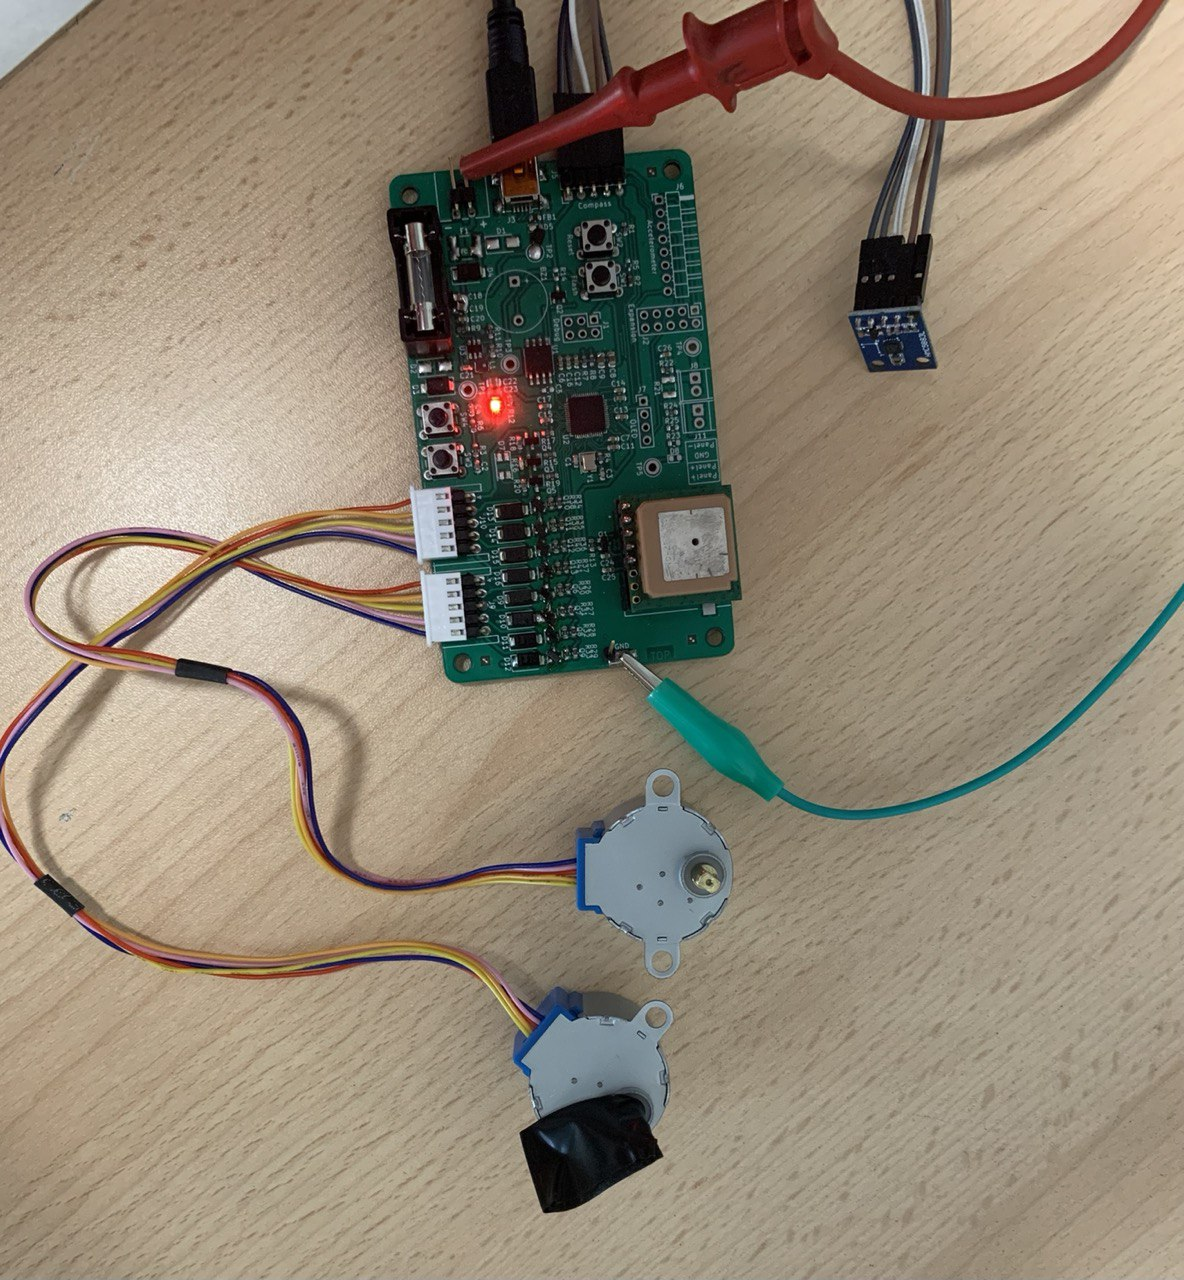
\includegraphics[scale=0.4]{figures/image101.png}
\captionsetup{type=figure}
\captionof{figure}{Scheda SALMO completa di componenti essenziali}
\end{center}

\noindent Abbiamo ripetuto questi passaggi per sei volte, realizzando così sei PCBA, uno per ogni membro del gruppo più uno per il professore.\\
Finito l’assemblaggio, ci siamo accorti che per una particolare scheda i pin del microcontrollore non sembravano 
essere fissati a dovere ed infatti testando la sua alimentazione abbiamo potuto constatare il surriscaldamento eccessivo 
del componente. Perciò per rimediare all’errore il microcontrollore è stato dissaldato, ma nel farlo, le tre piste che collegavano 
i rispettivi pin si sono alzate, non consentendo così l’utilizzo della scheda. Un altro errore è sorto durante la fase di testing, 
infatti, misurando il segnale di comando in input ai motori, ci siamo accorti che al transistor a canale N montato sulla scheda era 
stata assegnata la piedinatura scorretta. Pertanto, abbiamo dovuto dissaldare i transistor atti al pilotaggio dei motori per poi 
saldarli nuovamente nel verso corretto.

\begin{center}
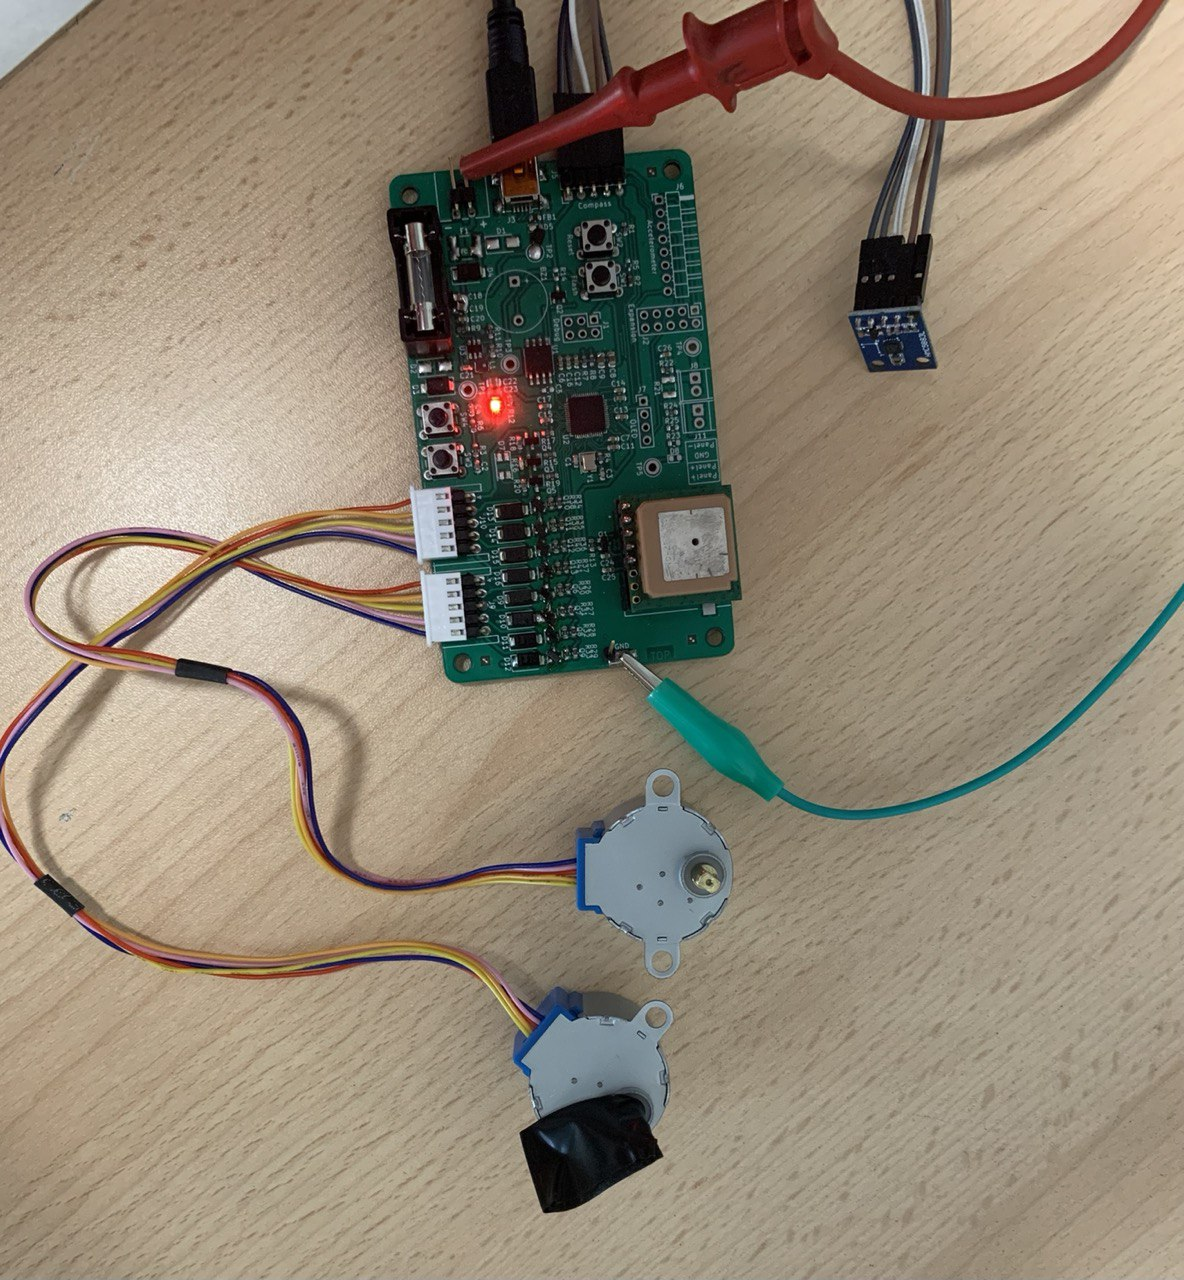
\includegraphics[scale=0.4]{figures/image101.png}
\captionsetup{type=figure}
\captionof{figure}{Scheda SALMO completa di componenti essenziali}
\end{center}